\section{Чем больше звуков, тем лучше? Аккорды}
\label{ch:harmony:chords}

Из раздела \ref{ch:harmony:interval} вы узнали, что \emph{интервал} для физиков --- это \emph{мера расстояния} между двумя звуками, а для лириков --- это \emph{два звука}, сыгранных одновременно или друг за другом.

Аккорд же --- понятие целиком лирическое.

\begin{Definition}[Аккорд]
    \emph{Аккорд}\index{аккорд} --- это три или более музыкальных звука, извлеченных (звучащих) одновременно.
\end{Definition}

Один из самых распространенных способов музыкального сопровождения песни (аккомпанемента\index{аккомпанемент}) --- игра так называемым <<боем>>. Правая рука ходит вверх-вниз, и ритмично бьет по \emph{всем} струнам одним или несколькими пальцами. Говорить о том, что звуки извлекаются одновременно не приходится --- струны задеваются одна за другой, но так как это происходит достаточно быстро, то \emph{звучат} они некоторое время все вместе и мы слышим \emph{аккорд}.

Есть ли правила построения гармонично звучащих аккордов?

Да, система аккордов сложилась и давно устоялась. Она определяет интервальную структуру аккордов и правила их именования, а в её основе лежат мажорный и минорный лады. Во всем множестве аккордов ярко выделяются две большие группы: мажорные (веселые) и минорные (грустные).

\begin{figure}[!ht]
    \centering
    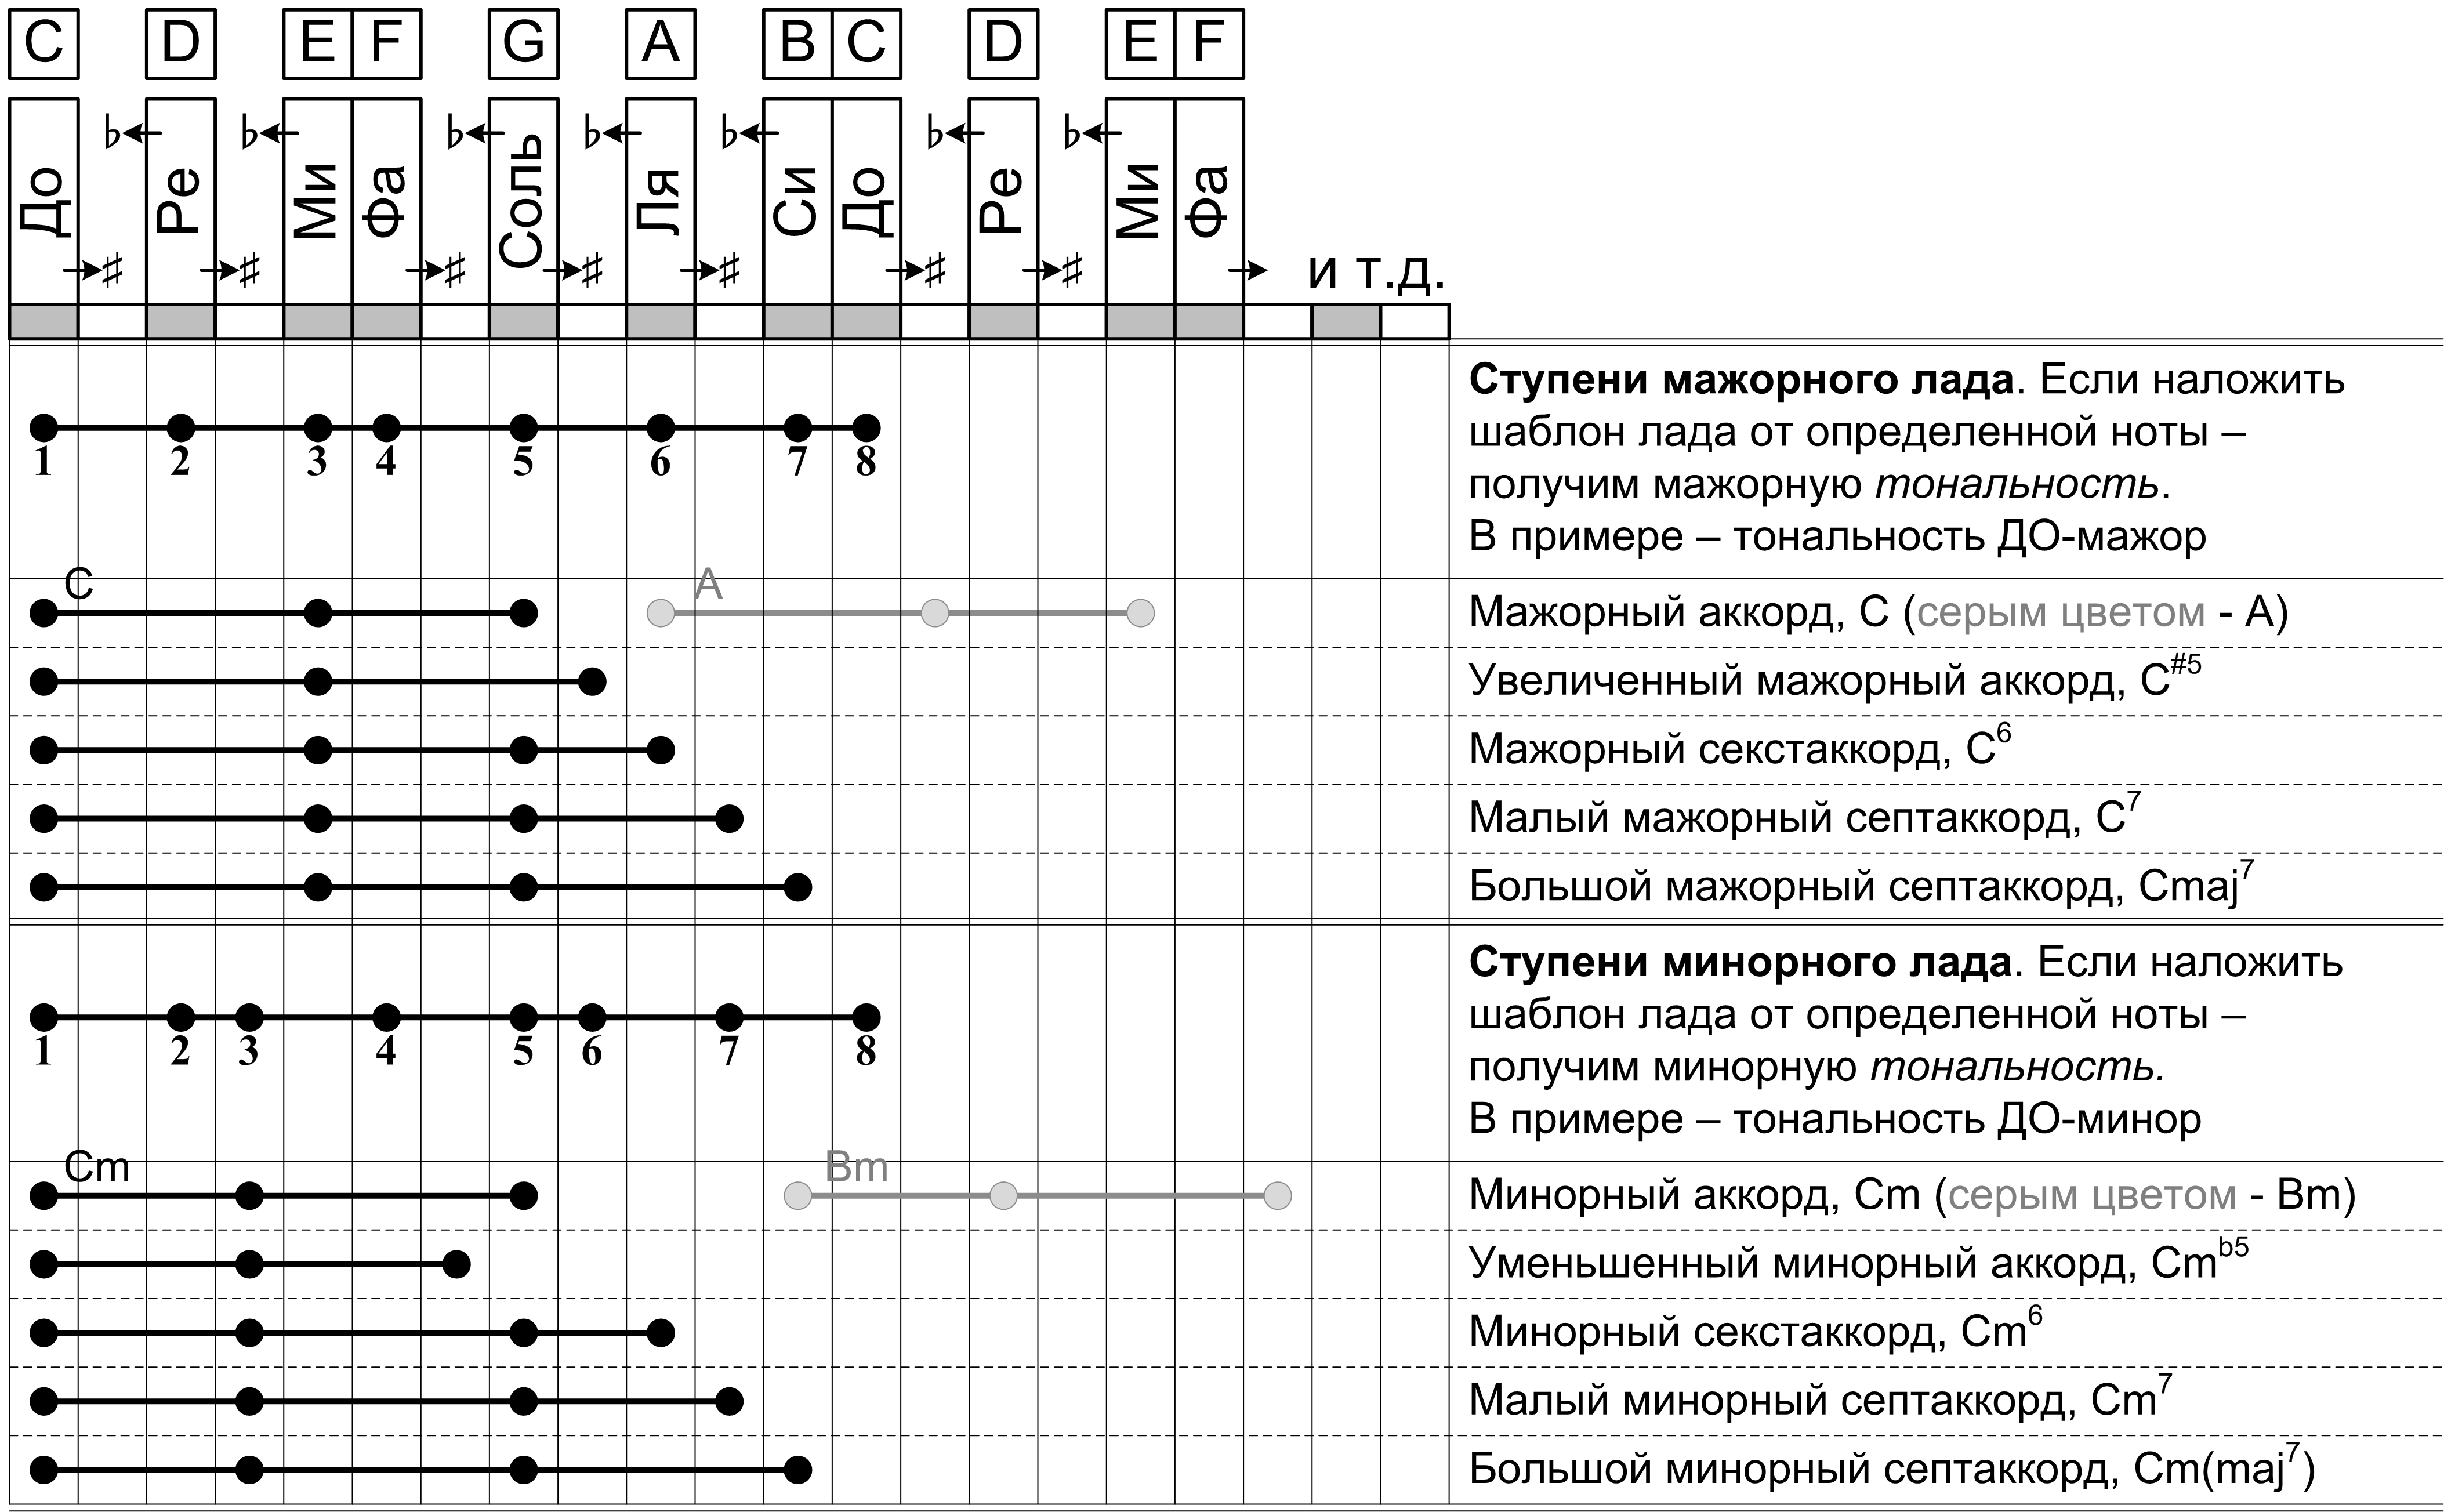
\includegraphics[width=\textwidth]{fig/chords/structure} 
    \caption{Интервальная структура некоторых аккордов}\label{fig:harmony:chords:structure}
\end{figure} 

Например, давайте рассмотрим интервальню структуру простого мажорного аккорда. Взгляните на рисунок \ref{fig:harmony:chords:structure}. В мажорный аккорд входят три музыкальных звука, на которые попадают соответственно первая, третья и пятая ступени мажорного лада. Первый, самый низкий, звук аккорда называется <<основным тоном>>\footnote{В западной терминологии основной тон аккорда называют root. Корень, источник. Все чаще и Русские люди называют основной тон <<корнем>> аккорда. А некоторые уважаемые люди (\cite{url:pimalive}) даже \emph{тоникой} аккорда!} аккорда. Второй звук будет отстоять от певого на 4 полутона, а третий от второго --- на 3 полутона. Интервальная структура мажорного аккорда:
\[
    \texttt{0-4-3}.
\]

Основной тон аккорда\index{тон основной!аккорда} --- нота, от которой строится аккорд, определяет его название. Допустим, мы откладываем шаблон мажорого аккорда от ноты ДО (С). Получившееся трезвучие будет называться <<ДО-мажор>>, и в его состав войдут ноты: 
\[
    \text{ДО}\xrightarrow{4}
    \text{МИ}\xrightarrow{3}
    \text{СОЛЬ}
\]

Домисолька\index{ДОМИСОЛЬКА}! Это не только название известного деткого музыкального театра города Москвы, но и веселый (мажорный) аккордик от ноты ДО! 

Аккорды принято обзначать в более короткой нотации. Так например, чтобы обозначить мажорный аккорд, просто используют латинское обозначение ноты основного тона. Домисолька будет обозначена кратко: <<C>>. А <<ЛЯ-мажор>>, в который входят ноты (см. рисунок \ref{fig:harmony:chords:structure}) ЛЯ(A), ДО-диез (C\#), МИ(E) будет обозначен как <<A>>.

Приведем краткий справочник обозначений и интервальных структур наиболее популярных\footnote{Описание полной системы аккордов выходит за скромные рамки этой книги. Нам важно общий принцип понять, а справочной информации об аккордах в Интернете --- завались} типов аккордов с жалкими попытками найти логику в их обозначениях (не забывайте поглядывать на рисунок \ref{fig:harmony:chords:structure}). Вместо $X$ смело подставляйте латинское обозначение любой из 12-ти нот октавы:

\begin{itemize}
    \item $X$ --- мажорный аккорд\index{аккорд!мажорный}. Состоит из трех нот, попадающих на 1, 3 и 5-ю ступени мажорного лада. Основа основ, нужно знать. Структура: \texttt{0-4-3}
    \item $X_m$ --- минорный аккорд\index{аккорд!минорный}. Те же три ступени, но минорного лада. Чтобы испольнить большинство <<гитарных>> песен, достаточно научиться играть мажорный и минорный аккорды. \texttt{0-3-4}

    \item $X^{\sharp 5}$ --- увеличенный мажорный аккорд. Смотрим на обозначение: это мажорный аккорд, у которого повышена на полутон пятая ступень мажорного лада (знак диез перед цифрой $\sharp 5$). \texttt{0-4-4}.
    \item ${X_m}^{\flat 5}$ --- уменьшенный минорный аккорд. Минорный аккорд с пониженной на полтона 5-й ступенью минорного лада. \texttt{0-3-3}.

    \item $X^6$ --- мажорный секстаккорд. Взяли мажорный аккорд и добавили четвертую нотку: 6-ю ступень мажорного лада. \texttt{0-4-3-2}. А вот называют <<секст>>-аккордом потому, что добавленный звук с основным тоном аккорда образует интервал <<секста>> (см. раздел \ref{ch:harmony:interval}).
    \item ${X_m}^6$ --- минорный секстаккорд. То же самое с минором. \texttt{0-3-4-2}.

    \item $X^7$ --- малый мажорный септаккорд (доминантсептаккорд). Взяли мажорный аккорд и добавили звук на расстоянии <<малой септимы>> от основного тона аккорда (напомню, малая септима --- пониженная на полтона 7-я стумень мажорного лада). \texttt{0-4-3-3}
    \item ${X_m}^7$ --- малый минорный септаккорд. No comments: \texttt{0-3-4-3}

    \item $X_{maj^7}$ --- большой мажорный септаккорд\index{аккорд!септаккорд}. Добавили к мажорному трезвучию большую септиму. \texttt{0-4-3-4}.
    \item $X_{m(maj^7)}$ --- большой минорный септаккорд. \texttt{0-3-4-4}.
\end{itemize}

Стоит отметить, что в оформлении обозначений аккордов особого единства нет. Например, <<ФА-малый мажорный септаккорд>> могут обозначить: $F_7$, $F^7$, а то и просто $F7$. Но разобраться можно. Помните только, что числа в обозначениях --- это ступени соответствующего лада.

Теперь подойдем поближе к гитаре. Кроме вопроса: <<А как зажать нужные струны?>>, возникает много вопросов. В простейших аккордах (например, в мажорном или минорном) три звука, а на гитаре 6 струн. Как же играют песни аккордами на гитаре <<боем>>? Бьют вроде по всем струнам, а звучит только три звука? Непонятно\ldots

Дело в том, что гитара не только \emph{устроена} с умом, но ещё и с умом \emph{настроена}! Настройте гитару классическим строем\footnote{Если возникают сложности с настройкой, обратитесь к разделу \ref{ch:guitar:tuning}}: МИ, СИ, СОЛЬ, РЕ, ЛЯ, МИ и давайте разбираться как <<ставить>> аккорды в первой позициии.

Что еще за позиции такие? Эх, оставьте на время эротические фантазии, тут все прозаично: позиция --- это номер лада на грифе, на который ставится (или может быть поставлен) указательный палец левой руки гитариста. Если вы, дожив до прочтения этих строк, сохранили большую часть пальцев левой руки, то в первой позиции вы сможете зажимать струны по крайней мере на четырех ладах, с 1-го по 4-й.

Давайте самостоятельно построим\index{аккорд!построение аппликатуры} аппликатуры нескольких аккордов. 

Начнем с аппликатуры аккорда $G$ --- <<СОЛЬ-мажор>>. Накладываем шаблон аккорда на ноту СОЛЬ (G), и определяем входящие в его состав ноты: СОЛЬ --- основной тон, СИ (В) и РЕ (D). Основной тон должен быть самым <<басистым>> поэтому важно найти ноту основного тона на басовых струнах (лучше на 6-й, но в крайнем случае можно и на 4-й). Нам везет: СОЛЬ находится на 3-м ладу 6-й струны --- в пределах первой позиции. На пятой струне в пределах первой позиции выбор невелик: только нота СИ. На 4-й струне мы вообще экономим палец --- её зажимать не надо, на открытой 4-й струне звучит нужная нам нота РЕ. Еще одна экономия: на открытой 3-й струне также звучит нота СОЛЬ (пусть октавой выше --- это ничего, она сольется с обертонами СОЛЬ на 6-й струне). Вторую струну можно оставить открытой (СИ), а можно зажать на 3-м ладу (РЕ). И, наконец, первую струну придется зажимать на 3-м ладу, чтобы получить еще одну СОЛЬ.

С местами прижатия определились. Рисуем аппликатурный бокс, отмечаем точки прижатия, берем гитару и подбираем удобные варианты расположения пальцев. В итоге должны получиться результаты как на рисунке \ref{fig:harmony:chords:G-variants}. Над аппликатурными боксами дополнительно изображена нотная запись аккордов: первые три аккорда --- чистые СОЛЬ-мажор трезвучия в разных октавах, а последние два аккорда --- шесть звуков, которые получатся, если сыграть наши аппликатуры <<боем>> по всем шести струнам. Но как уже было сказано, эти шесть звуков прозвучат как трезвучие мажорного аккорда, потому что три \emph{верхних} звука сольются в абсолютном консонансе со звуками (т.е. <<утонут>> в их обертонах), которые \emph{ниже} их на октаву (или две).

\begin{figure}[!ht]
    \centering
    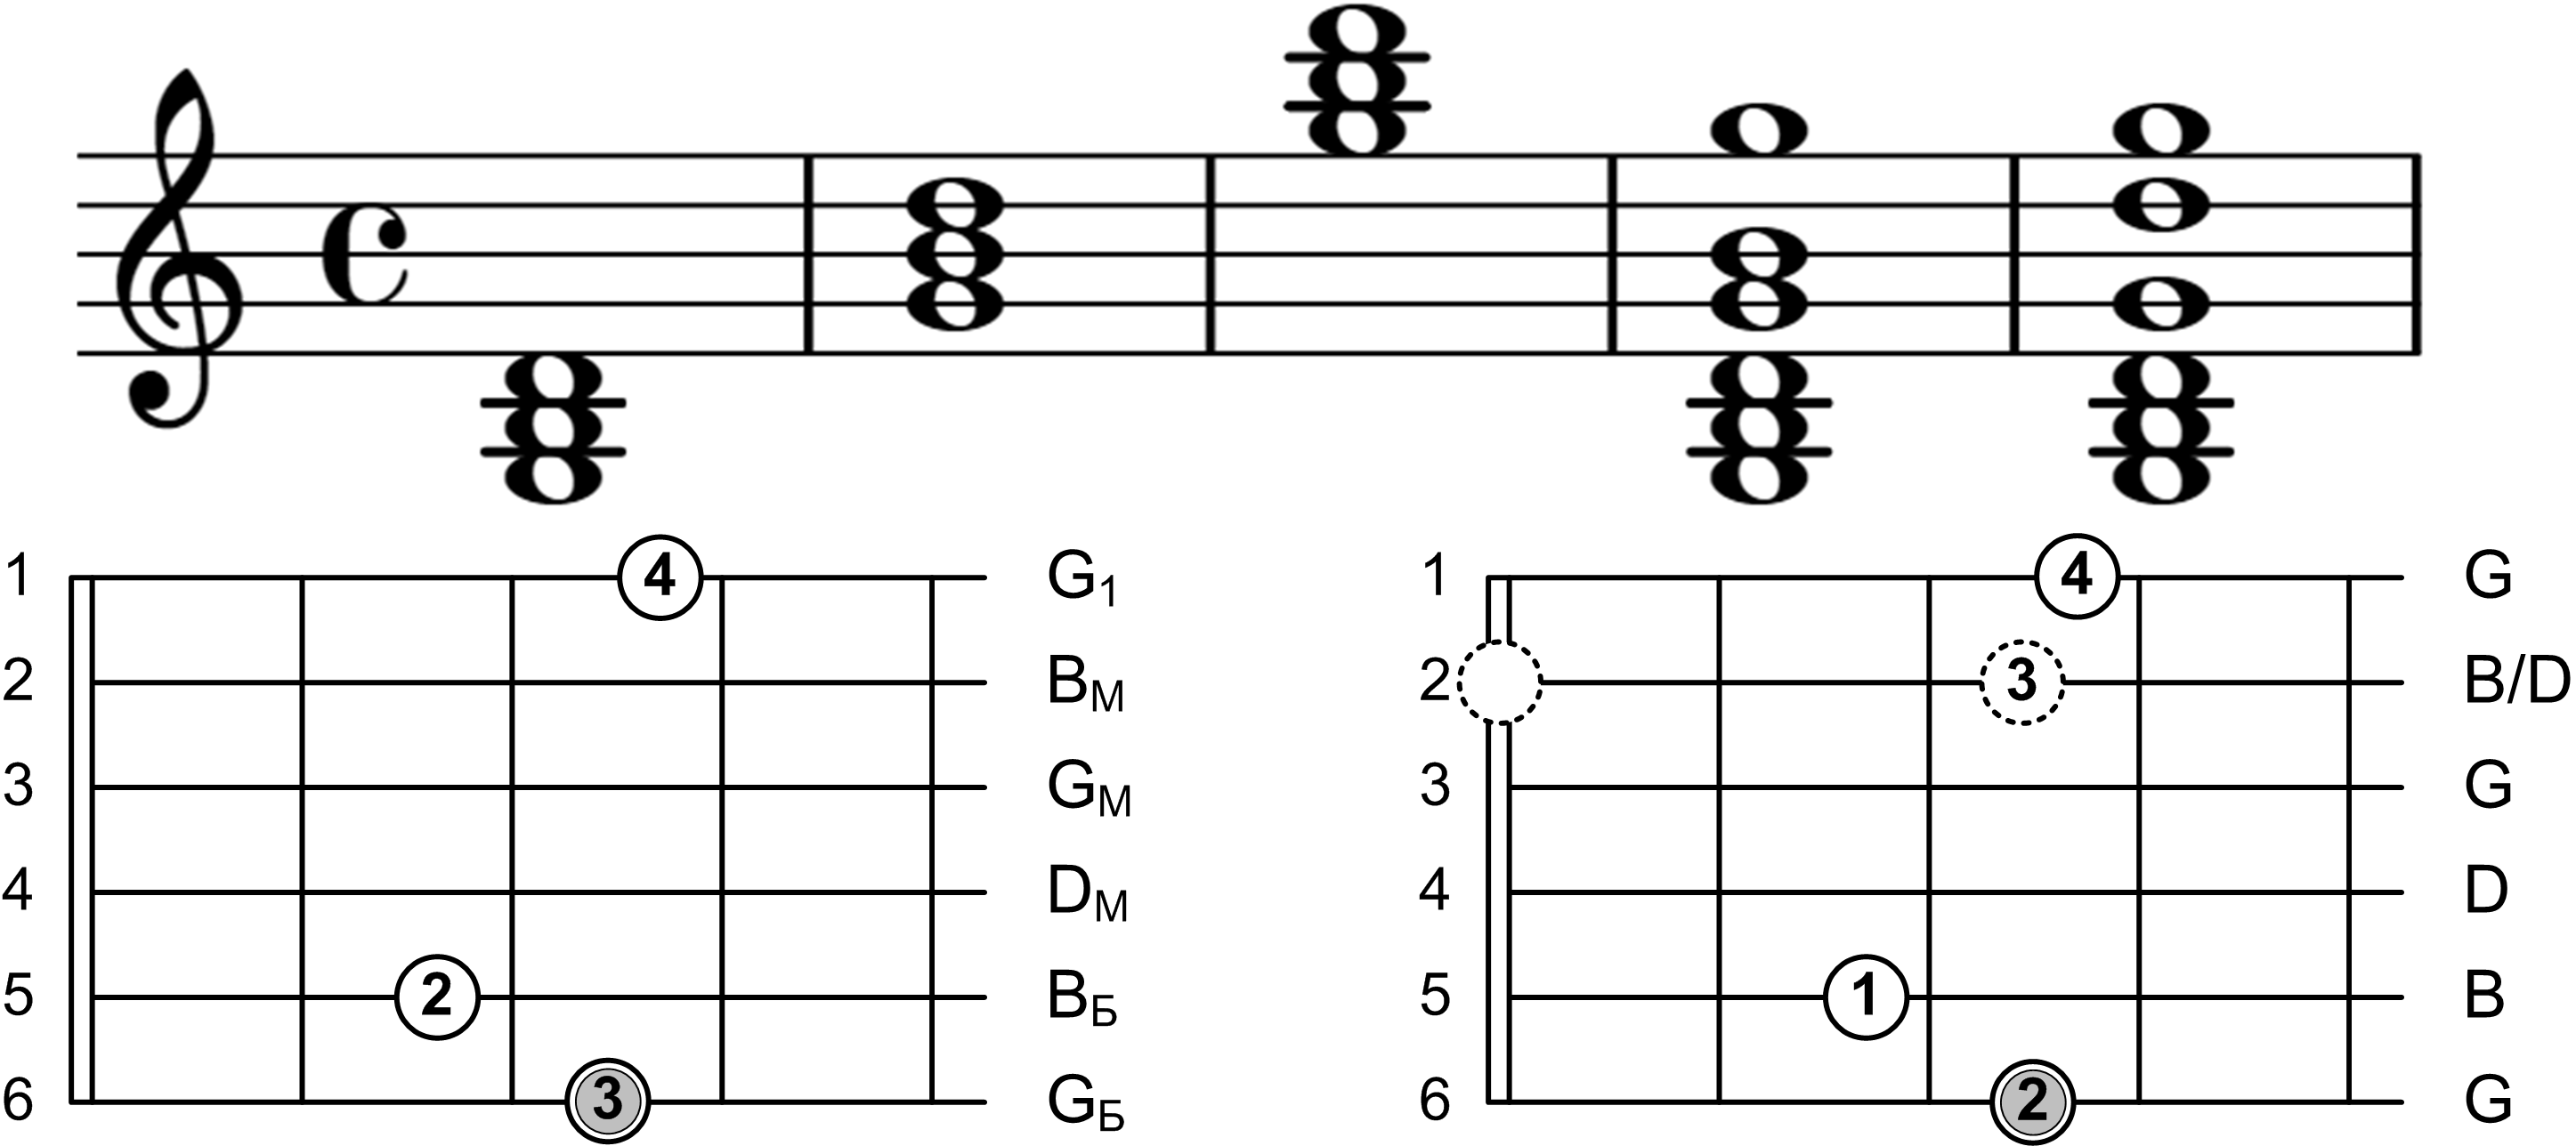
\includegraphics{fig/chords/G-variants} 
    \caption{Возможные варианты аппликатур аккорда $G$ (СОЛЬ-мажор)}\label{fig:harmony:chords:G-variants}
\end{figure} 

Аппликатурные боксы\index{бокс аппликатурный} аккордов обычно изображают фрагмент грифа в 4-5 ладов. Слева от бокса иногда пишут номера струн, сверху (если это аккорд не в первой позиции) --- номера ладов. Точки прижатия струн обозначают кружками. Точку прижатия основного тона всегда выделяют, мы будем делать это серым кружком с двойной белой рамкой. Номера пальцев пишут  внутри кружков. Мы (пока) справа от бокса будем также писать латинские обозначения звучащих на струне нот. Если на струне может быть несколько вариантов прижатия, то они будут обозначены пунктирными кружками. Если струна в аккорде звучать категорически \emph{не должна}, то её будем перечеркивать над самым верхним порожком. Если струна своим звуком портит аккорд, но несильно, и <<\emph{лучше бы ей не звучать, но если и прозвучит, то ничего страшного}>>, то над самым верхним порожком над струной будем ставить кружок со знаком вопроса.

На рисунке \ref{fig:harmony:chords:G-variants} аппликатура аккорда $G$ слева является <<канонической>>, но она сложна для начинающих, так как требует хорошей растяжки между 3 и 4-м пальцами. Однако, к тому времени когда эта аппликатура не будет представлять сложности, музыкант поймет, что именно она позволяет экономно <<перескочить>> в аппликатуры других аккордов (например в $C$). Аппликатуру справа проще поставить, кроме того, она позволяет использовать третий палец, чтобы добавить в аккорд нотку РЕ(D) вместо СИ(B), что многие находят более красивым.

Чтобы минорным аккордам было не обидно, построим аппликатуру в первой позиции для аккорда <<ЛЯ-минор>>, который составляют ноты: ЛЯ --- основной тон, ДО и МИ. Начинаем с басовых струн и находим основной тон только на открытой пятой струне. В этом случае шестую струну \emph{лучше не трогать, но в принципе можно}, так как на ней (открытой) звучит МИ, которая вообще не испортила бы этот аккорд, если бы не звучала <<басистее>> основного тона, что, конечно, нехорошо. На втором ладу четвертой струны находим МИ, на втором ладу третьей --- ЛЯ, на первом ладу второй --- ДО, на открытой первой --- МИ. Вариантов получается немного, см. рисунок \ref{fig:harmony:chords:Am}. 

\begin{Example}[Эксперимент с аккордом $A_m$]
    Мы построили аккорд ЛЯ-минор (см. рисунок \ref{fig:harmony:chords:Am}), особенностью которого является то, что шестую струну <<лучше бы>> не трогать.
    
    Поставьте аккорд левой рукой, а большим пальцем правой руки проведите по всем струнам сверху-вниз. Звучит немного <<подпорченный>> с теоретической точки зрения аккорд $A_m$, потому что самый низкий звук аккорда --- МИ на шестой струне, а не ЛЯ, как должно быть. Слушаем, оцениваем.
    
    А теперь не трогайте шестую струну, проведите пальцем по струнам, начав с пятой струны. Теперь прозвучал во всех отношениях правильный $A_m$. Самый низкий звук аккорда, как и положено основной тон ЛЯ($A$).
\end{Example}

\begin{figure}[!ht]
    \centering
    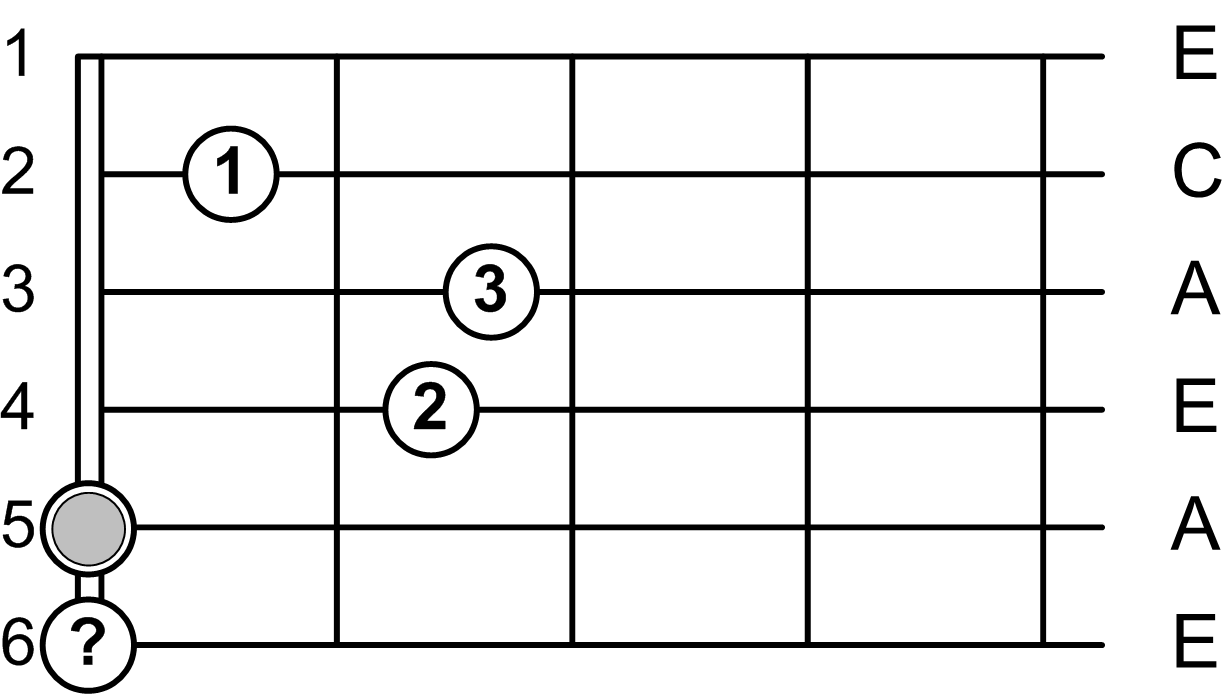
\includegraphics{fig/chords/Am} 
    \caption{Аппликатура аккорда $A_m$ (ЛЯ-минор)}\label{fig:harmony:chords:Am}
\end{figure} 

В качестве разминки попробуйте построить аппликатуру аккорда $D_m$. Его аппликатура приведена на рисунке \ref{fig:harmony:chords:Dm}. Сверьтесь и ответьте на вопрос: <<почему нельзя трогать шестую струну?>>

\begin{figure}[!ht]
    \centering
    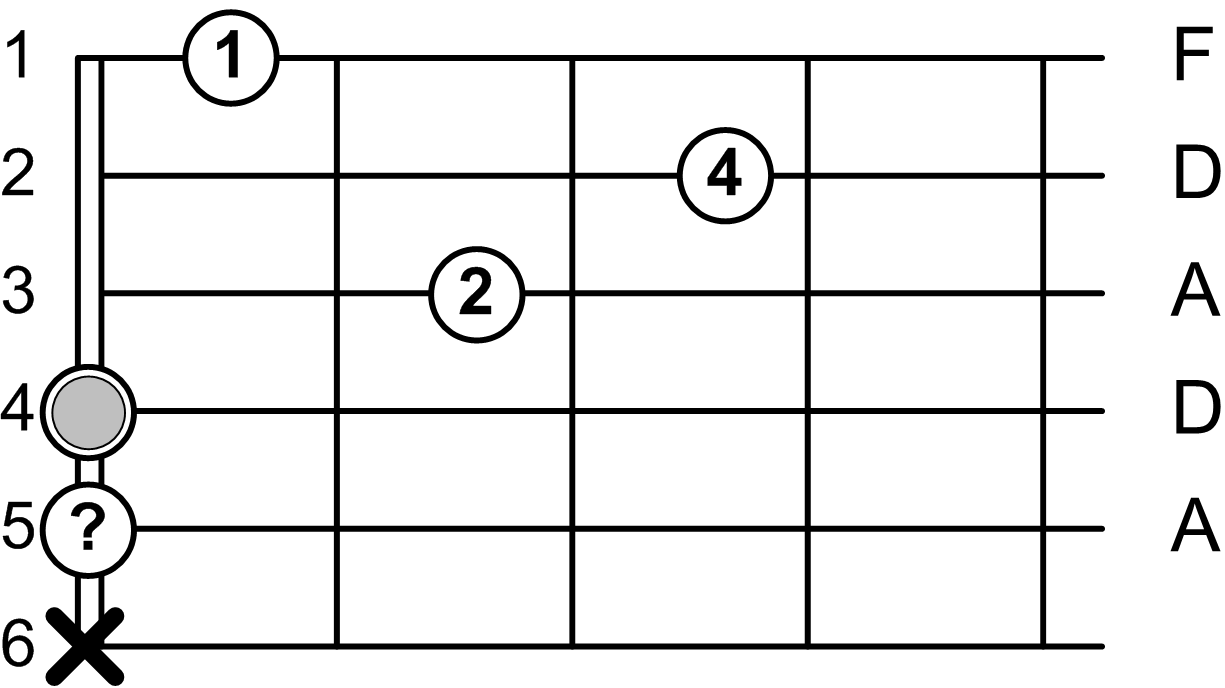
\includegraphics{fig/chords/Dm} 
    \caption{Аппликатура аккорда $D_m$ (РЕ-минор)}\label{fig:harmony:chords:Dm}
\end{figure} 

Готовые аппликатуры аккордов несложно найти: есть и справочники, и множество ресурсов в сети Интернет. Но имейте в виду, что, найдя аппликатуру, неплохо бы уметь проверить её <<на вшивость>> --- от ошибок ведь никто не застрахован. Вы теперь сумеете. Возможно когда-нибудь вы дойдёте до таких вершин мастерства, что решите использовать нестандартный строй гитары и стандартные аппликатуры в тот же миг превратятся в мусор. Но вы уже сейчас знаете как построить аппликатуру аккорда, а к тому времени ваш мозг сможет построить её мгновенно, <<на лету>>.

На рисунке \ref{fig:harmony:chords:popular} приведены аппликатуры наиболее популярных аккордов в первой позиции, зная которые, вы сможете сыграть музыкальное сопровождение (аккомпанемент) к большинству популярных песен.

\begin{figure}[!ht]
    \centering
    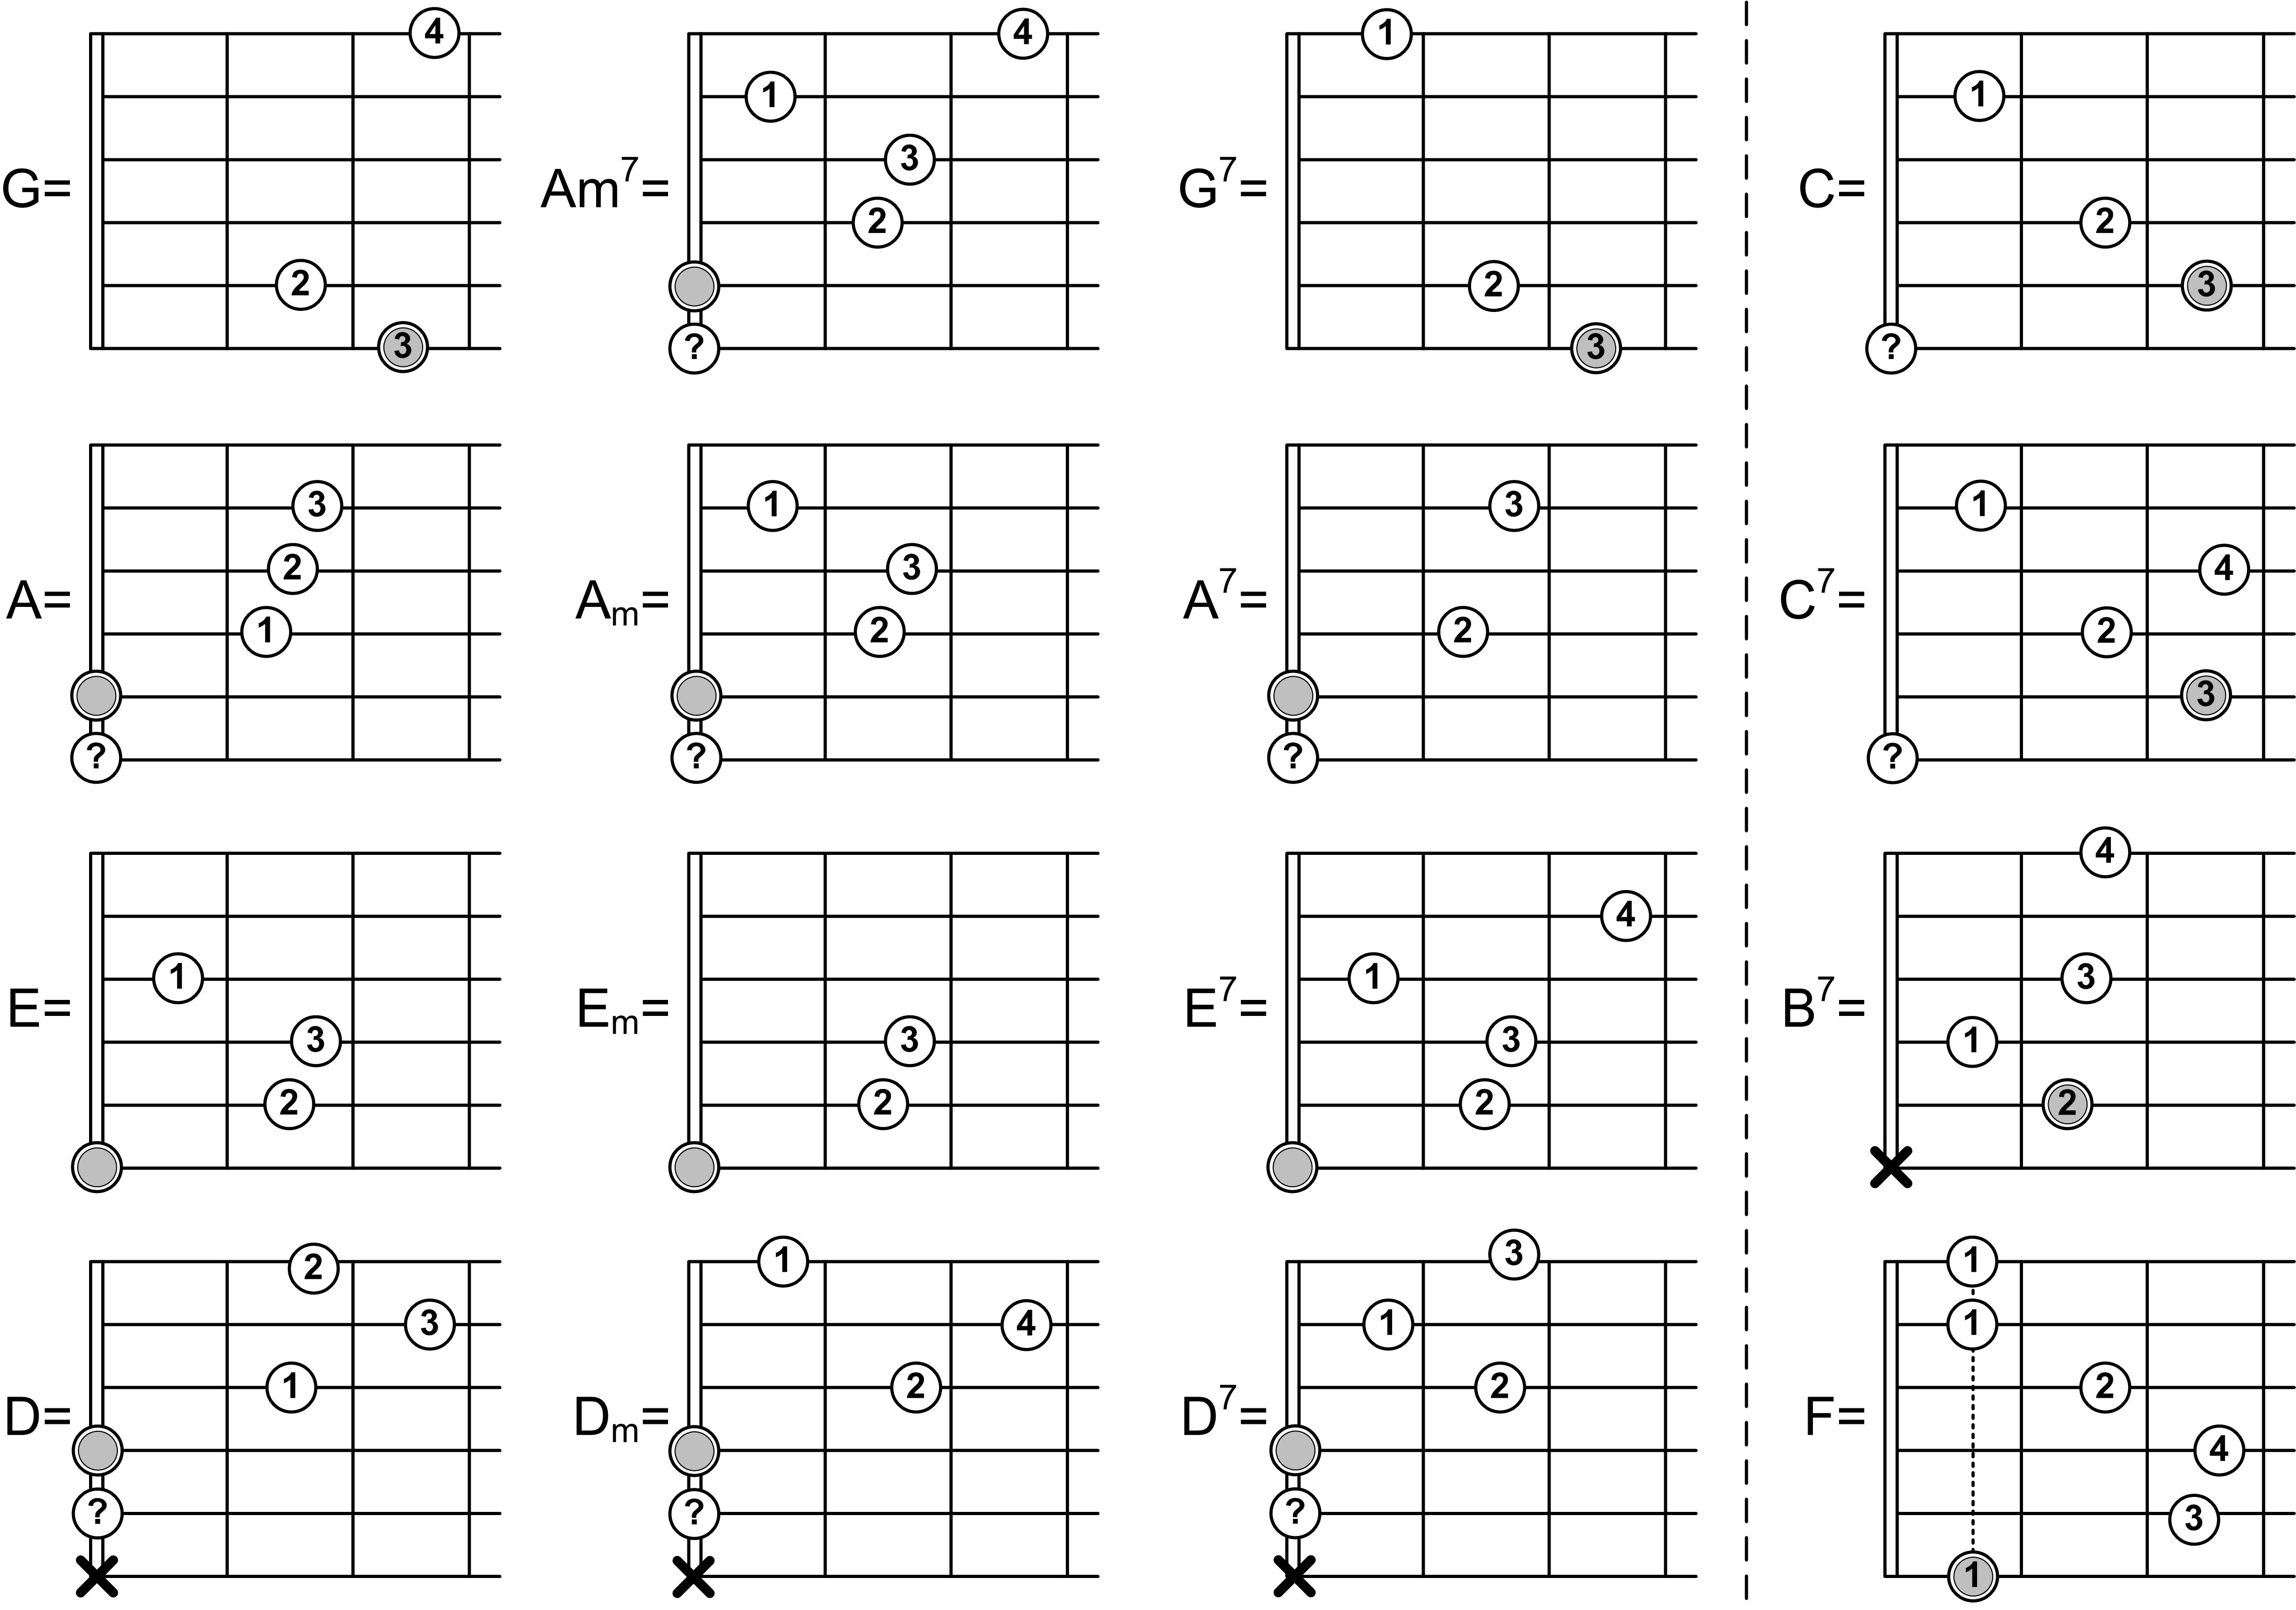
\includegraphics{fig/chords/popular} 
    \caption{Аппликатуры популярных <<песенных>> аккордов}\label{fig:harmony:chords:popular}
\end{figure} 

Можно подумать, что аккорды существуют только в первой позиции! Конечно, нет. Задумайтесь над тем, что произойдет, если вы просто сместите точки прижатия струн для любого аккорда в первой позиции на $n$ ладов вниз по грифу? Тип аккорда не изменится, так как сохранится относительное положение звуков (т.е. интервальная структура останется прежней). Например, как был аккорд малым мажорным септаккордом, так им и останется. А вот основной тон аккорда будет повышен на $n$ полутонов! Теоретически, нам достаточно научиться <<сдвигать>> аккорды из первой позиции вниз по грифу, а не сидеть и придумывать новую аппликатуру.

На практике такой сдвиг бывает сложно сделать, потому что на левой руке всего пять пальцев, а желательно бы иметь семь (шесть со стороны струн, плюс большой). В первой позиции нам активно помогал экономить пальцы верхний порожек: нет нужды ставить палец, если нужная нота и так звучит на открытой струне! Если же мы просто сместим кисть на $n$ ладов, то верхний порожек останется там, где и был: часть неприжатых струн будет звучать как и звучала до сдвига, а не на $n$ полутонов выше, как требуется.

И тут на сцену выходит \emph{указательный} палец левой руки и говорит: <<Роль передвижного верхнего порожка буду играть я! Я знаю крутой прием, называется \emph{баррэ}\index{баррэ}! Только подберите аппликатуру в первой позиции попроще, чтобы оставшиеся три пальца справились>>.

Рассмотрим прием <<сдвига>> аккорда\index{аккорд!сдвиг}. Например, нам хочется сыграть <<ЛЯ-минор>> ($A_m$) с основным тоном на 5-м ладу 6-й струны. Обращаем свой взор на легкие аппликатуры минорных аккордов в первой позиции (см. хотя-бы рисунок \ref{fig:harmony:chords:popular}), у которых основной тон на 6-й струне. Кажется, $E_m$ (МИ-минор) идеально подходит! На рисунке \ref{fig:harmony:chords:shift} детально изображен процесс <<сдвига>> аккорда $E_m$ в аккорд $A_m$. Структура прижатий осталась, а вот положение пальцев пришлось изменить: указательный (1-й) палец исполняет прием <<баррэ>>\index{баррэ}, прижимая все струны к 5-му ладовому порожку, а 3 и 4-й пальцы зажимают на 7-м ладу 5 и 4-ю струны соответственно. Получившуюся аппликатуру можно <<носить>> по всему грифу, получая минорные аккорды практически с любым основным тоном: начиная от ФА-минор, когда баррэ на первом ладу, и заканчивая той позицией в основании грифа, на которую сил и гибкости хватит.

\begin{figure}[!ht]
    \centering
    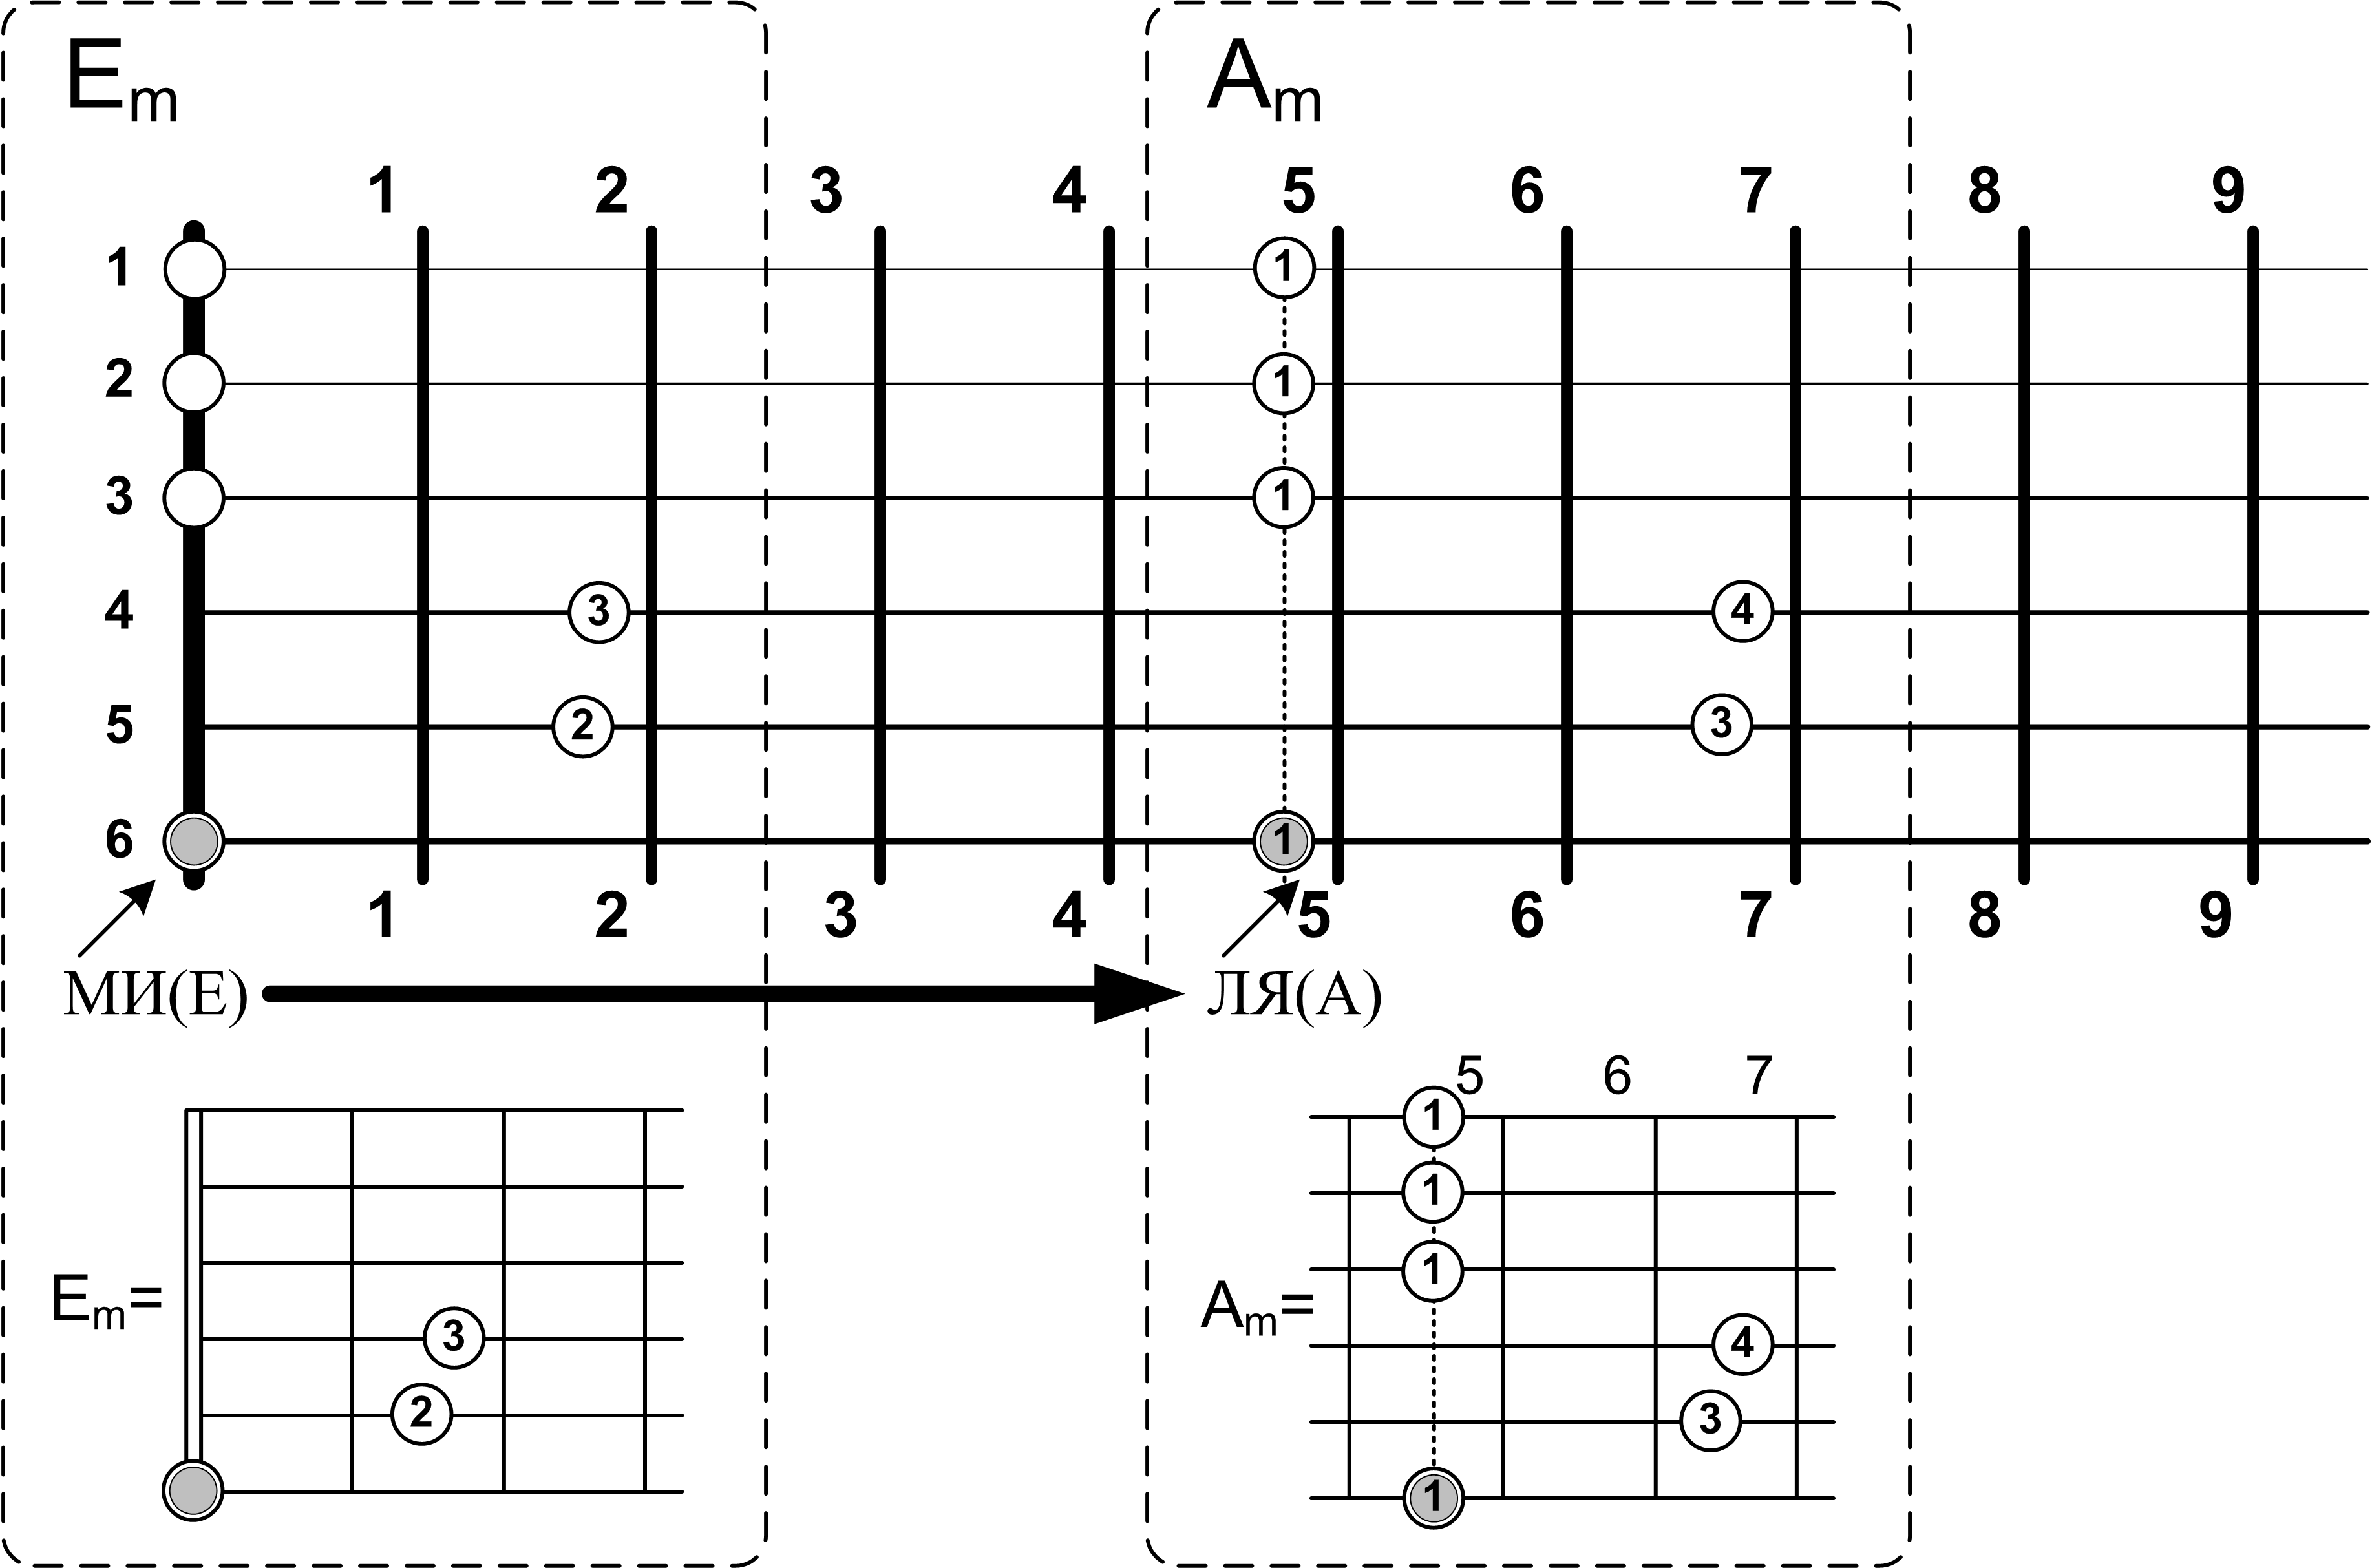
\includegraphics[width=\textwidth]{fig/chords/shift} 
    \caption{Сдвиг аккорда\index{аккорд!сдвиг} $E_m$ из первой позиции в аккорд $A_m$}\label{fig:harmony:chords:shift}
\end{figure} 


Мораль вышеизложенного: изучите аппликатуры первой позиции для интересующих вас аккордов. Запоминайте наиболее легкие варианты. Потом, когда вы откроете психоделический, пестрящий картинками, справочник аккордов, вы всегда увидите сдвинутую форму аппликатуры первой позиции, и вам сильно полегчает. Например, обратите внимание на аккорд $F$ на рисунке \ref{fig:harmony:chords:popular}, в котором используется прием баррэ, --- ничего не напоминает?
